\textbf{The Algorithm:} The Augmented-UCB (AugUCB) algorithm is presented in Algorithm~\ref{alg:augucb}.
AugUCB is essentially based on the arm elimination method of the UCB-Improved \cite{auer2010ucb}, but adapted to the thresholding bandit setting proposed in \cite{locatelli2016optimal}. However, unlike the UCB improved (which is based on mean estimation) our algorithm employs \emph{variance estimates} (as in \cite{audibert2009exploration}) for arm elimination; to the best of our knowledge this is the first variance-aware  algorithm for the thresholding bandit problem. Further, we allow for arm-elimination at each time-step, which is in contrast to the earlier work (e.g., \cite{auer2010ucb,chen2014combinatorial}) where the arm elimination task is deferred to the end of the respective exploration rounds. The details are presented below.

% In algorithm \ref{alg:augucb}, hence referred to as AugUCB, we have two exploration parameters, $\rho_{\mu}$ and $\rho_v$ which are the arm elimination parameters. $\psi_{m}$ is the exploration regulatory factor. 
%The main approach is based on the UCB-Improved algorithm with modifications suited for the thresholding bandit problem. 
The active set $B_{0}$ is initialized with all the arms from $\mathcal{A}$. We divide the entire budget $T$ into rounds/phases like in UCB-Improved, CCB, SAR and CSAR. At every time-step AugUCB checks for arm elimination conditions, while updating parameters at the end of each round. As suggested by \cite{liu2016modification} to make AugUCB to overcome too much early exploration, we no longer pull all the arms equal number of times in each round. Instead, we choose an arm in the active set $B_m$ that minimizes $(|\hat{r}_{i} - \tau |-2s_i)$ where 
%$\min_{i\in B_{m}}\big\lbrace |\hat{r}_{i} - \tau | - 2\sqrt{\frac{\rho_v\psi_m \hat{V}_{i} \log ( T \epsilon_{m})}{4 n_{i}} + \frac{\rho_v\psi_m \log{( T\epsilon_{m})}}{4 n_{i}}} \big\rbrace $
\begin{small}
\begin{align*}
s_i & = \sqrt{\frac{\rho\psi_m (\hat{v}_{i}+1) \log ( T \epsilon_{m})}{4 n_{i}}} %+ \frac{\rho\psi_m \log{( T\epsilon_{m})}}{4 n_{i}}}.
\end{align*}
\end{small} 
with $\rho$ being the arm elimination parameter and $\psi_{m}$ being the exploration regulatory factor.
%  in the active set $B_{m}$. 
The above condition ensures that an arm closer to the threshold $\tau$ is pulled; 
%and with suitable choice of $\rho_{\mu}$ and $\rho_v$ we can fine tune the exploration. 
parameter $\rho$ can be used to fine tune the elimination interval.
The choice of exploration factor, $\psi_m$,
% $\psi_m=\frac{T\epsilon_m}{(\log(\frac{3}{16} K\log K))^{2}}$ 
comes directly from \cite{audibert2010best} and \cite{bubeck2011pure} where it is  stated that in pure exploration setup, the exploring factor must be linear in $T$ (so that an exponentially small probability of error is achieved) rather than being logarithmic in $T$ (which is more suited for minimizing cumulative regret).

\begin{algorithm}[t!]
\caption{AugUCB}
\label{alg:augucb}
\begin{algorithmic}
\State {\bf Input:} Time budget $T$; parameter $\rho$; 
% $\rho_{\mu}$, $\rho_v$ 
  threshold $\tau$
\State {\bf Initialization:} $B_{0}=\mathcal{A}$; $m=0$; $\epsilon_{0}=1$;
\begin{small}
\begin{align*}
M&=\left\lfloor \frac{1}{2}\log_{2} \frac{T}{e}\right\rfloor; 
\hspace{2mm}\psi_{0}=\frac{T\epsilon_{0}}{128\Big(\log(\frac{3}{16}K\log K)\Big)^2}; \\
\ell_{0}&=\left\lceil \frac{2\psi_0\log( T\epsilon_{0})}{\epsilon_{0}} \right\rceil;
\hspace{2mm}N_{0}=K\ell_{0}
\end{align*}
\end{small}
%$M=\left\lfloor \frac{1}{2}\log_{2} \frac{T}{e}\right\rfloor $,  
%$\psi_{0}=\frac{T\epsilon_{0}}{(\log(\frac{3}{16}K\log K)^2}$,
% $\ell_{0}=\left\lceil \frac{2\psi\log( T\epsilon_{0})}{\epsilon_{0}} \right\rceil$ and 
% $N_{0}=K\ell_{0} $. Pull each arm once.
\State Pull each arm once
\vspace{-2mm}
\State \For{$t=K+1,..,T$}
\State Pull arm $j\in\argmin_{i\in B_{m}}\Big\lbrace |\hat{r}_{i} - \tau | - 2s_{i}\Big\rbrace$
% \State where $s_j=\sqrt{\frac{\rho\psi_{m}\hat{v}_{j}\log{( T\epsilon_{m})}}{4 n_{j}} + \frac{\rho\psi_{m} \log{(T\epsilon_{m})}}{4 n_{j}}}$
\State $t\leftarrow t+1$ 
\vspace{-4mm}
%\ArmElim
%\State For each arm $i \in B_{m}$, remove arm ${i}$ from $B_{m}$ if
%\begin{align*}
%\hat{r}_{i} + c_i  < \tau - c_i \mbox{ or } \hat{r}_{i} - c_i  > \tau + c_i \\
%\text{where $c_i=\sqrt{\frac{\rho_{\mu}\psi_{m}\log{( T\epsilon_{m})}}{2 n_{i}}}$}
%\end{align*}
%\EndArmElim
%\ArmElimV
%\State \For{$i\in B_m$}
%\State For each arm $i \in B_{m}$, remove arm ${i}$ from $B_{m}$ if
\State \For{$i\in B_m$}
\vspace{-4mm}
\State \If{$(\hat{r}_{i} + s_i  < \tau - s_i)$ or $(\hat{r}_{i} - s_i > \tau + s_i)$}
\State $B_m\leftarrow B_m\backslash\{i\}$\hspace{4mm} (Arm deletion)
\EndIf
\EndFor
%\begin{align*}
%\hat{r}_{i} + s_i  < \tau - s_i,\hspace{1mm} \mbox{ or } \hspace{1mm}\hat{r}_{i} - s_i  > \tau + s_i \\
%% \text{where $s_i=\sqrt{\frac{\rho\psi_{m}\hat{v}_{i}\log{( T\epsilon_{m})}}{4 n_{i}} + \frac{\rho\psi_{m} \log{(T\epsilon_{m})}}{4 n_{i}}}$}
%\end{align*}
%\EndFor
%\EndArmElimV
\vspace{-2mm}
\State \If{$t\geq N_{m}$ and $m \leq M$}
%\ResetParam
\State \textbf{Reset Parameters}
\State $\epsilon_{m+1}\leftarrow\frac{\epsilon_{m}}{2}$
\State $B_{m+1} \leftarrow B_{m}$
\State $\psi_{m+1}\leftarrow \frac{T\epsilon_{m+1}}{128(\log(\frac{3}{16}K\log K))^{2}}$
\State $\ell_{m+1}\leftarrow\left\lceil \frac{2\psi_{m+1}\log( T\epsilon_{m+1})}{\epsilon_{m+1}} \right\rceil$
\State $N_{m+1} \leftarrow t + |B_{m+1}|\ell_{m+1}$
\State $m \leftarrow m+1$
%\EndResetParam
\EndIf
\EndFor
\State \textbf{Output:} $\hat{S}_{\tau}=\lbrace i: \hat{r}_{i}\geq \tau \rbrace$.
\end{algorithmic}
\end{algorithm}

A simplified illustrative flowchart highlighting the main steps of AugUCB is provided in Figure \ref{fig:augucb}. Also note the similarity between UCB-Improved (Figure \ref{fig:ucbimp}) and AugUCB in this flowchart.

\begin{figure}[!th]
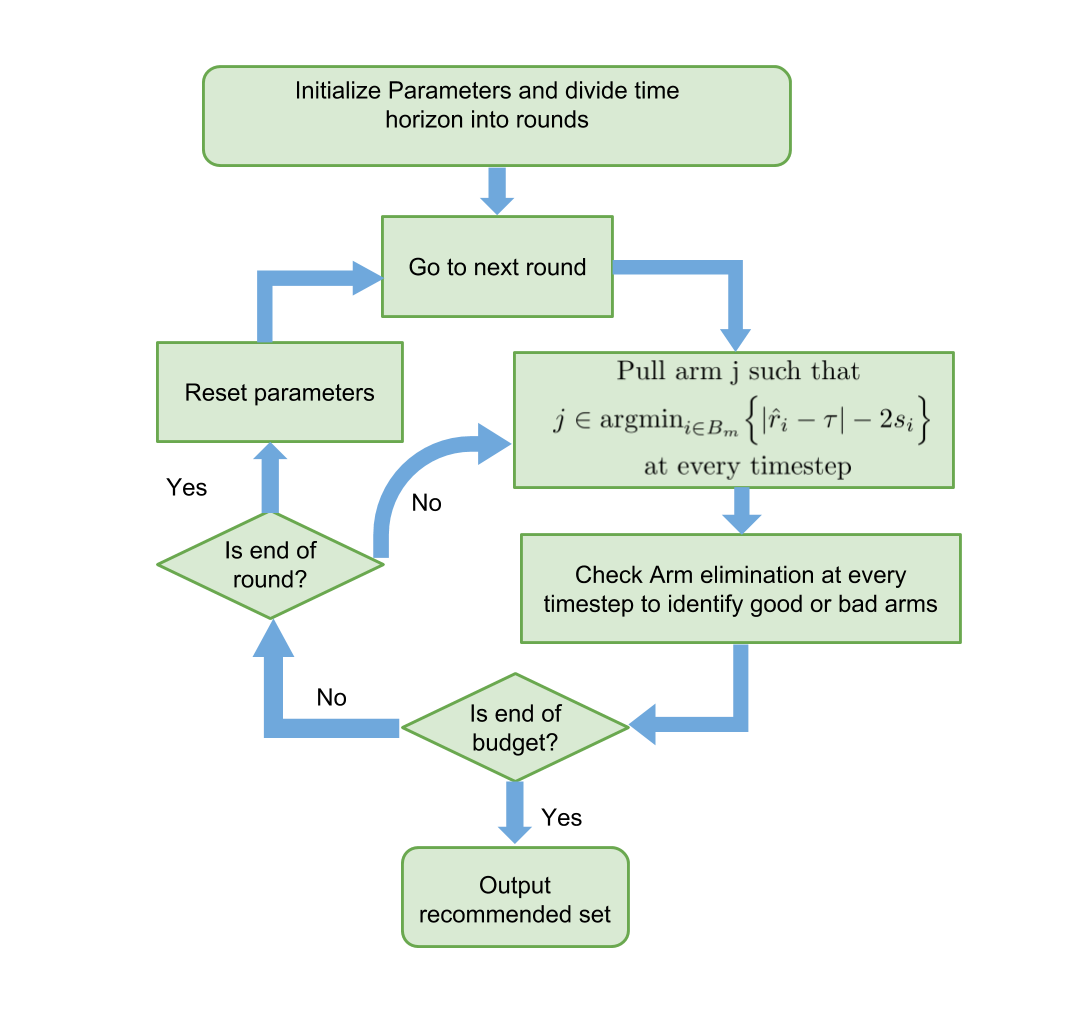
\includegraphics[scale=0.45]{Chapter5/img/AugUCB_flow.png}
\caption{Flowchart for AugUCB}
\label{fig:augucb}
\end{figure}


%Also because of the said condition, like \cite{liu2016modification} we also claim that AugUCB is an anytime algorithm.
